\documentclass[12pt]{article}
\usepackage[utf8]{inputenc}
\usepackage[T1]{fontenc}	
\usepackage{array,latexsym}
\usepackage{amsmath,amsfonts,amssymb,amsthm,mathabx,amstext}
\usepackage{dsfont}	% Conjuntos: $\mathds{N, Z, Q, R, C}$
\usepackage{graphicx}
\begin{document}
\pagestyle{empty}
\begin{center}
	UNIVERSIDADE FEDERAL DA PARAÍBA\\
	Introdução à Álgebra Linear\\
	Primeira Prova\\
	Paulo Ricardo Seganfredo Campana - 20210044220\\
\end{center}

Questão 1.\\
1.) Subespaço vetorial é um subconjunto não vazio de um Espaço vetorial tal que a soma de dois vetores desse subespaço e que a multiplicação de um vetor por um escalar também estará contido no subespaço.\\
$u+v\in W, \forall u,v\in W$\\
$\alpha u \in W, \forall u \in W, \alpha \in \mathds{R}^{3}$\\\\
2.) Sim, pois não é vazio e:\\
$(x,0,0)+(y,0,0)=(x+y,0,0)$ que $\in W$\\
$\alpha (x,0,0) = (\alpha x,0,0)$ que $\in W$\\\\
3.) Não, pois na multiplicação por um escalar $\alpha$ não inteiro, a matriz deixa de seguir a regra imposta deste subespaço.\\\\
4.) Sim, pois não e vazio e:\\
$(0+a_{1}x+a_{2}x^{2}+a_{3}x^{3}) + (0+b_{1}x+b_{2}x^{2}+b_{3}x^{3}) =$\\ 
$(0+(a_{1}+b_{1})x + (a_{2}+b_{2})x^{2}+(a_{3}+b_{3})x^{3})$ que $\in W$\\
$\alpha(0+a_{1}x+a_{2}x^{2}+a_{3}x^{3}) = (0 + \alpha a_{1}x+\alpha a_{2}x^{2}+\alpha a_{3}x^{3})$ que $\in W$\\\\

Questão 2.\\
$W = [(1,2,3)(1,-1,1)] = (x+y,2x-y,3x+y)$\\
$U = (x,y,0)$\\
$\left\{\begin{array}{@{}l@{}}
	x+y=x\\
	2x-y=y\\
	3x+y=0
\end{array}\right. \Longrightarrow x=y=0$\\
$U\cap W = (0,0,0)$\\\\

Questão 3.\\
$\begin{bmatrix}1&-5\\-5&5\end{bmatrix}=
a\begin{bmatrix}1&-1\\-1&2\end{bmatrix}+
b\begin{bmatrix}4&1\\1&0\end{bmatrix}+
c\begin{bmatrix}3&-2\\-2&1\end{bmatrix}$\\
$\left\{\begin{array}{@{}l@{}}
	a+4b+3c=1\\
	-a+b-2c=-5\\
	-a+b-2c=-5\\
	2a+c=5
\end{array}\right. $\\
Escalonando...\\
$a=2,\quad b=-1,\quad c=1$\\
$[\begin{bmatrix}1&-5\\-5&5\end{bmatrix}]_{\alpha} = \begin{bmatrix}2&-1\\-1&1\end{bmatrix}$\\\\


Questão 4.\\
1.)\\
$U = (x,y,z,2z-y)$\\
$\beta_{U} = [(1,0,0,0),(0,1,0,-1),(0,0,1,2)]$\\
$W = (x,2z,z,x)$\\
$\beta_{W} = [(1,0,0,1),(0,2,1,0)]$\\
$U\cap W = \left\{\begin{array}{@{}l@{}}
	x=t\\
	y=2z\\
	t=2\-y
\end{array}\right.$\\
$t=2z-2z \Longrightarrow t = 0 \Longrightarrow x = 0$\\
$U\cap W = (0,2z,z,0)$\\
$\beta_{U\cap W} = (0,2,1,0)$\\
2.)\\
$U+W = [(1,0,0,0),(0,1,0,-1),(0,0,1,2),(1,0,0,1),(0,2,1,0)]$\\
$(0,2,1,0)$ pode ser escrito como $2(0,1,0-1) + (0,0,1,2)$ então sera eliminado.\\
$\left\{\begin{array}{@{}l@{}}
	x=0\\
	y-t=0\\
	z+2t=0\\
	x+t=0
\end{array}\right. \Longrightarrow x = 0,\quad t = 0, \quad y = 0,\quad z =0$\\
São vetores LI e formam a base de $U+W$, portanto geram $U+W$ e formam soma direta de $\mathds{R}^{4}$\\

Questão 5.\\
1.)$\beta$ é uma base de um Espaço se $\beta$ é LI e $\beta$ gera o Espaço em questão.\\
2.) Sim, são LI:\\
$\left\{\begin{array}{@{}l@{}}
	x+y=0\\
	y+2z=0\\
	y+z=0
\end{array}\right. \Longrightarrow z = -y$\\
$y-2y=0,\quad y=0$\\
$x+0=0,\quad x=0$\\
$z=-y,\quad z=0$\\
$\left\{\begin{array}{@{}l@{}}
	x+z=0\\
	x+y+2z=0\\
	x+2y+4z=0
\end{array}\right. \Longrightarrow z=-x$\\
$x+y-2x=0 \Longrightarrow y-x=0, \Longrightarrow x=y$\\
$x+2x-4x=0 \Longrightarrow x=0, \quad y=0, \quad z=0$\\\\
e geram $\mathds{R}^{3}$:\\
$(x,y,z)=a(1,1,0)+b(0,1,2)+c(0,1,1)$\\
$(x,y,z)=(a, a+b+c, 2b+c)$\\\\
$(x,y,z)=a(1,0,1)+b(1,1,2)+c(1,2,4)$\\
$(x,y,z)=(a+b+c, b+2c, a+2b+4c)$\\\\
3.)\\
a)\\
$\left\{\begin{array}{@{}l@{}}
	a=-1\\
	a+b+c=2\\
	2b+c=-5
\end{array}\right. \Longrightarrow a=-1$\\
$b+c-1=2 \Longrightarrow b+c=3$\\
$2b+c=-5 \Longrightarrow -2b-c=5$\\
$-b=8 \Longrightarrow b=-8$\\
$-16+c=-5 \Longrightarrow c =11$\\
$ [(-1,2,-5)]_{\alpha} = (-1,-8,11)$\\\\
$\left\{\begin{array}{@{}l@{}}
	a+b+c=-1\\
	b+2c=2\\
	a+2b+4c=-5
\end{array}\right.$\\
$-a-b-c=1,\quad + \quad a+2b+4c=-5 \Longrightarrow b+3c=-4$\\
$b+3c=-4,\quad + \quad -b-2c=-2 \Longleftarrow c=-6$\\
$b-18=-4, \Longrightarrow b = 14$\\
$a+14-6=1, \Longleftarrow a = -7$\\
$[(-1,2,-5)]_{\beta} = (-7,14,-6)$\\

b)\\
\begin{figure}[h!]
	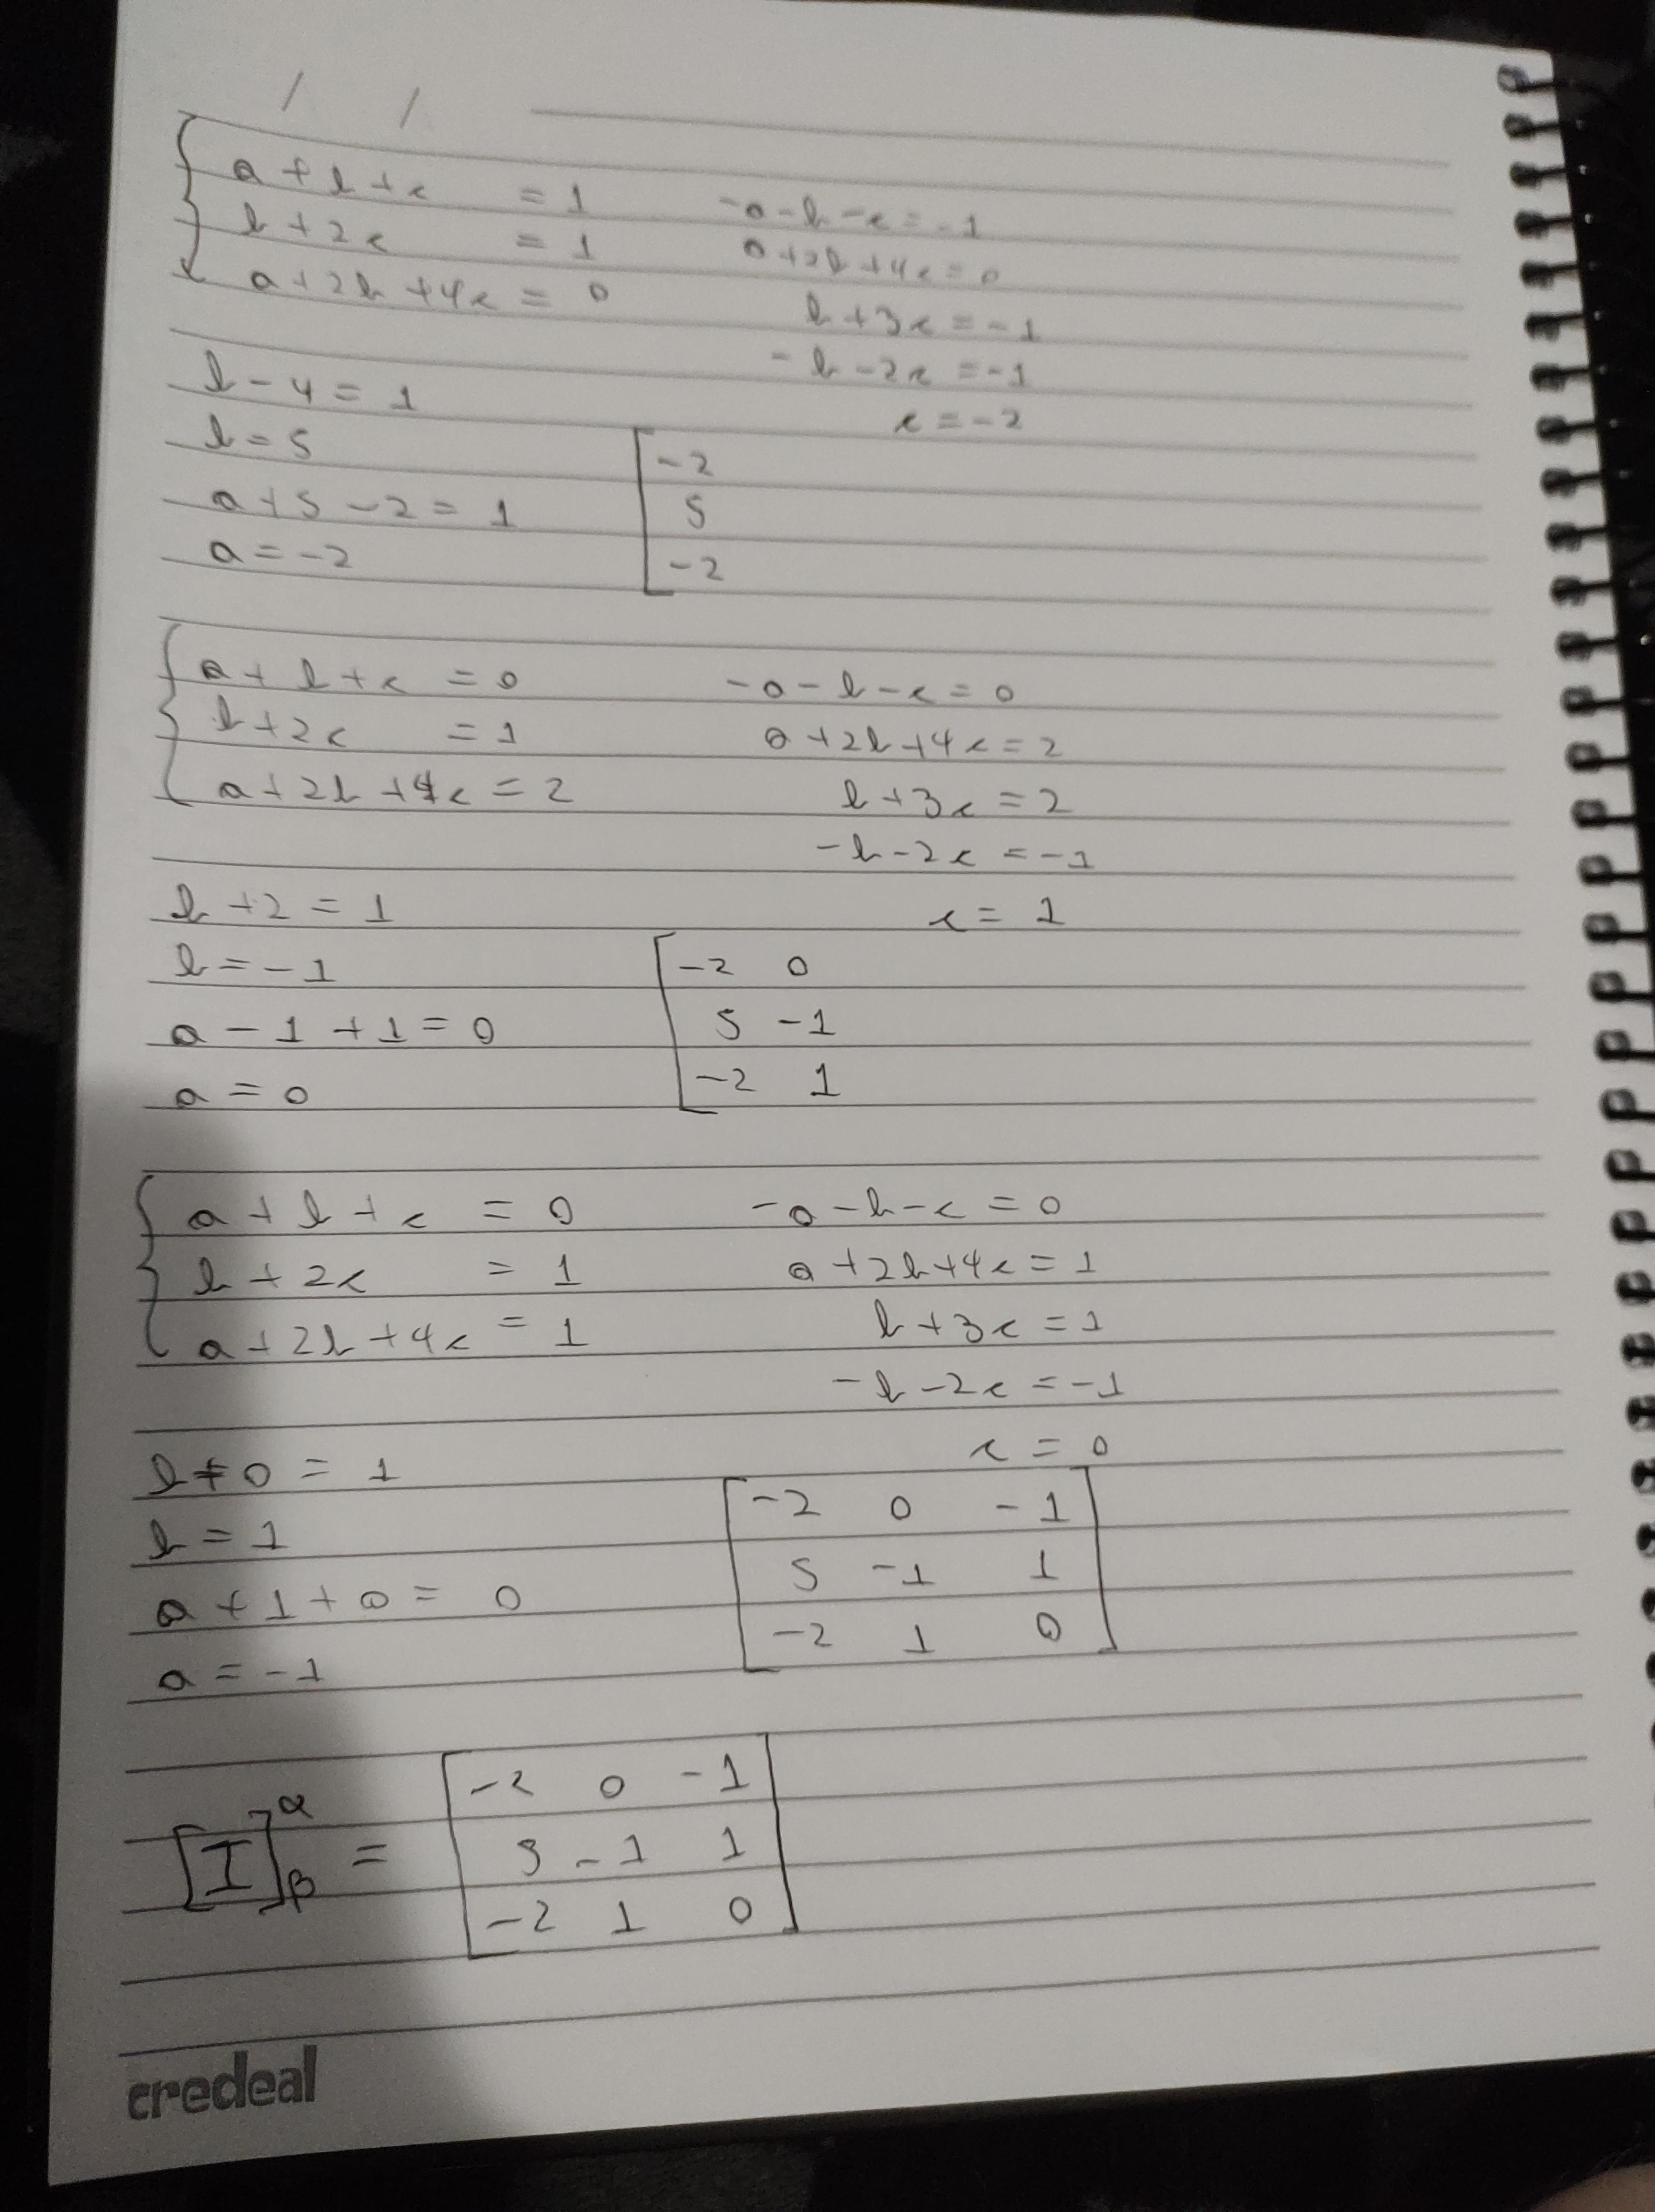
\includegraphics[scale=0.12]{q5a}
\end{figure}
\begin{figure}[h!]
	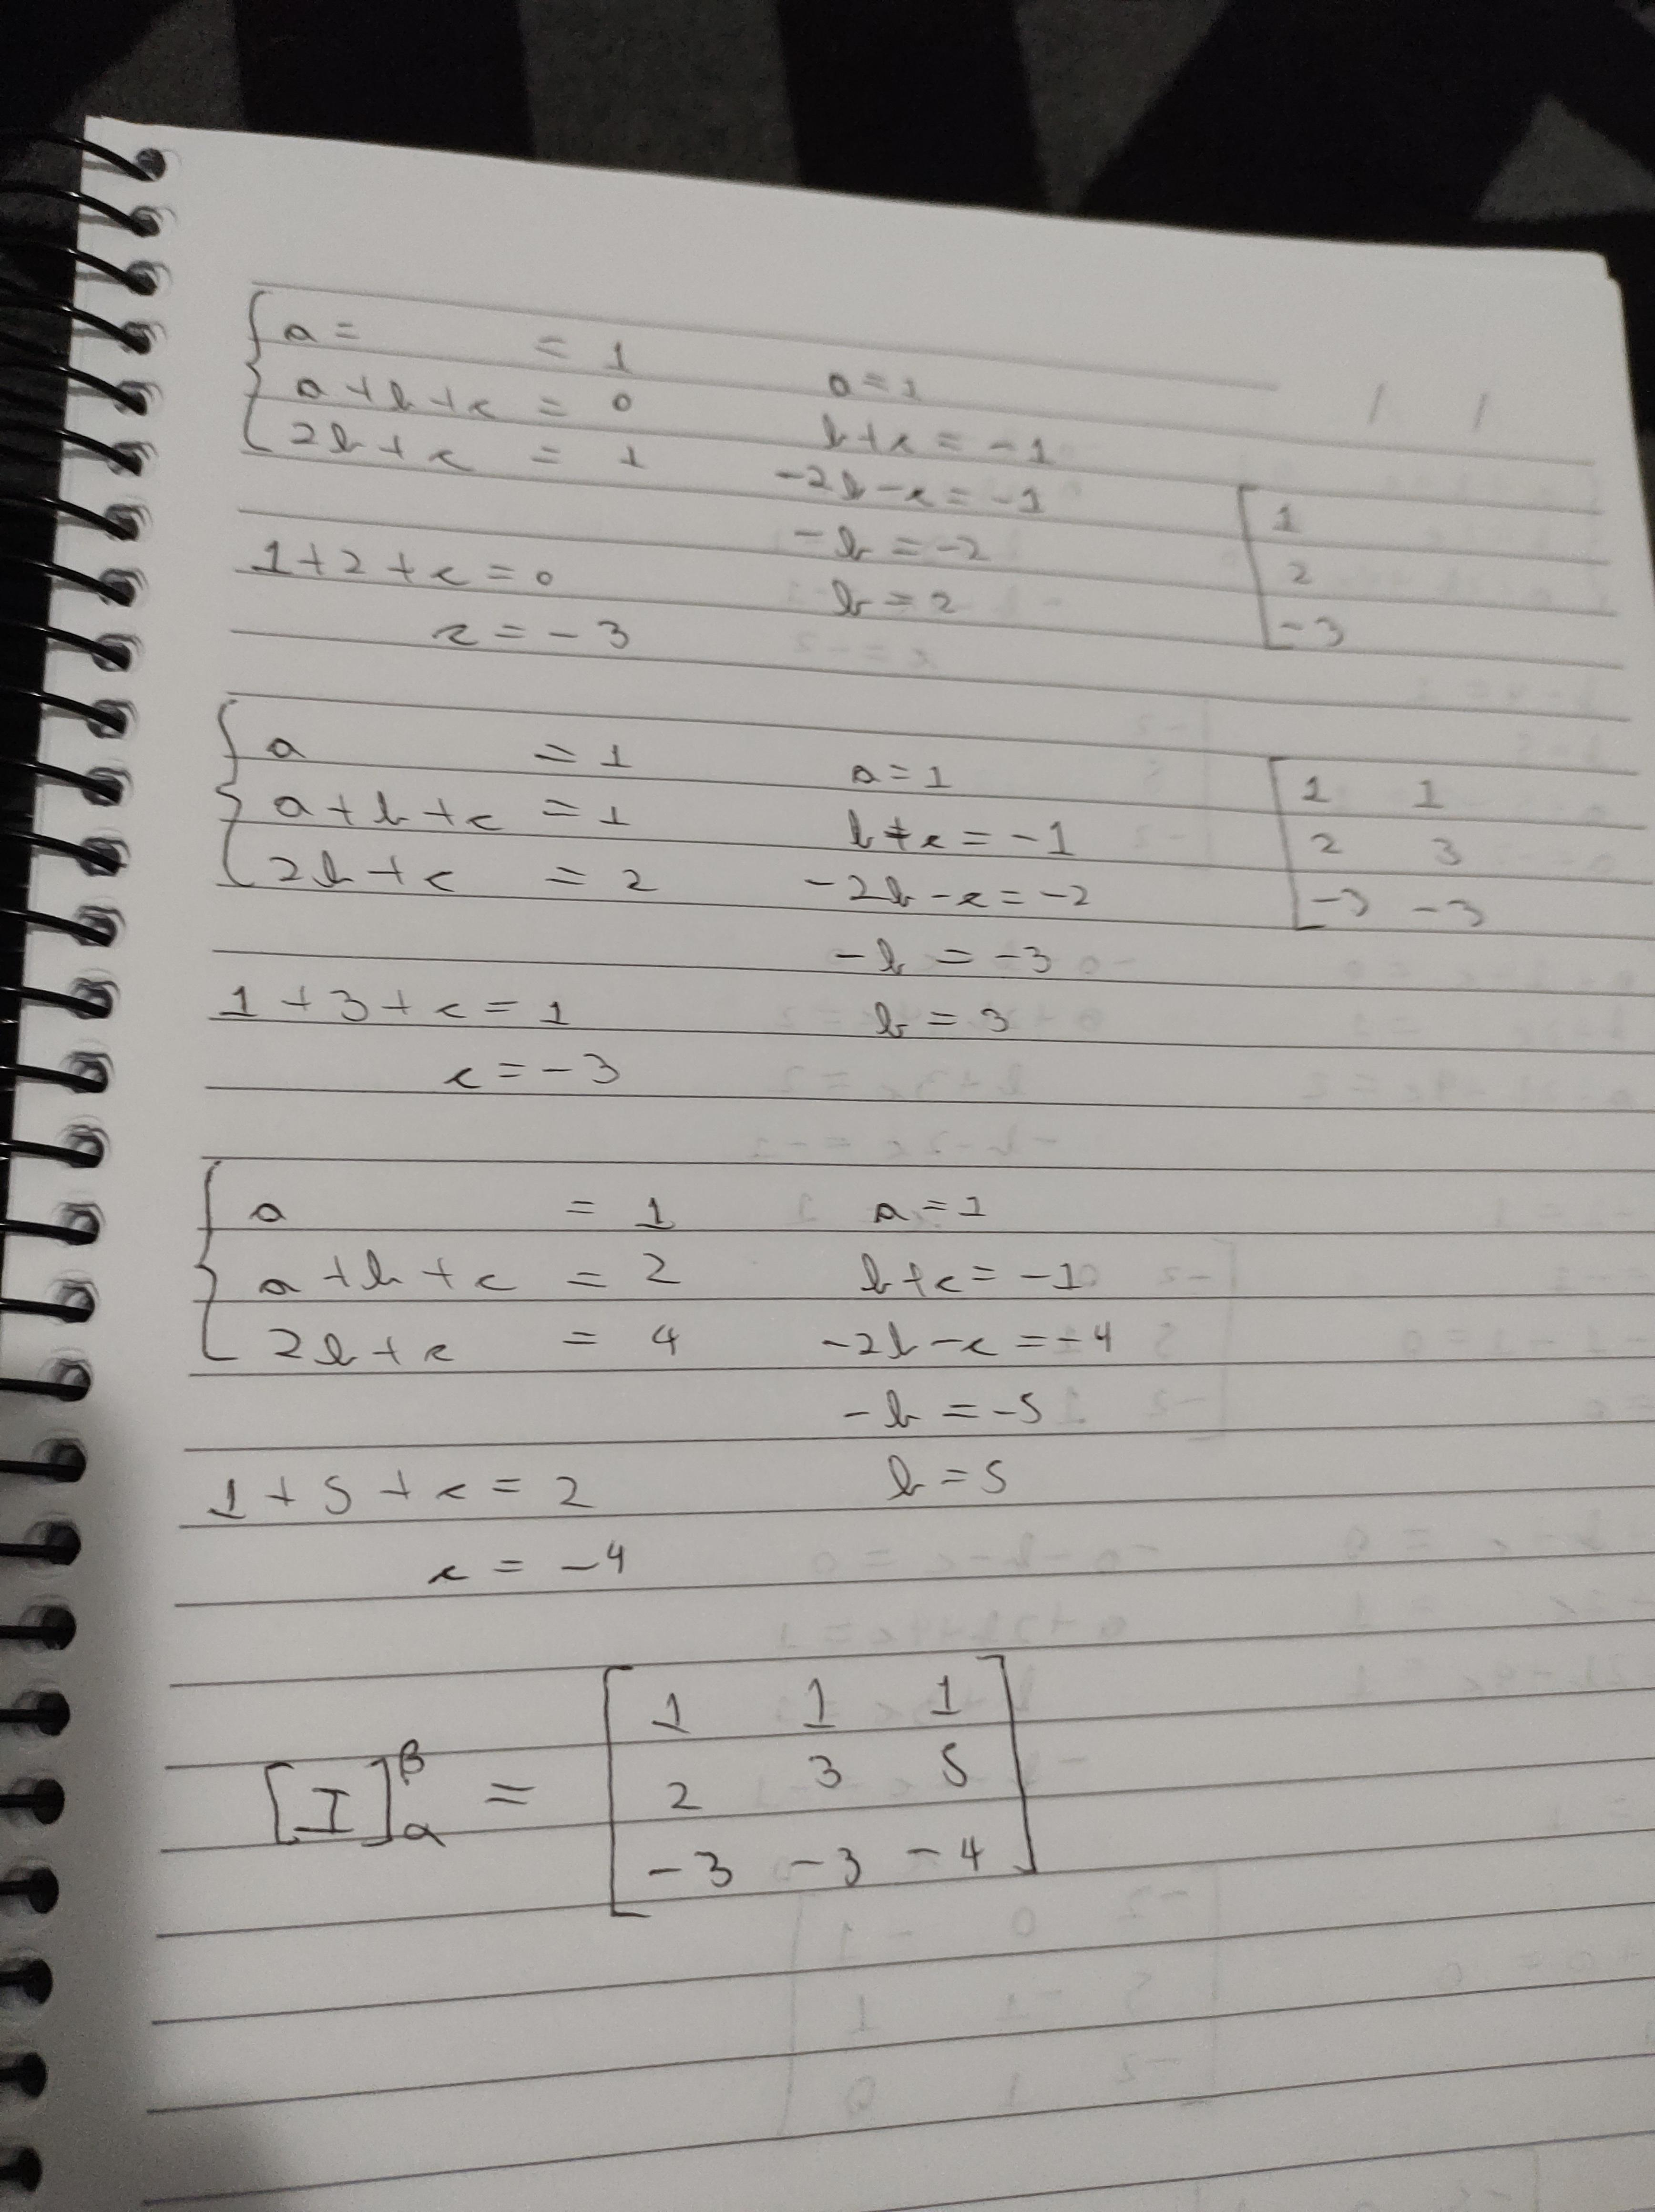
\includegraphics[scale=0.12]{q5b}
\end{figure}
c) Sim, pois $\displaystyle[[I]^{\beta}_{\alpha}]^{\alpha}_{\beta} = [I]$\\
















\end{document}